\documentclass[12pt]{article}
\usepackage{graphicx}
\usepackage{placeins}


% acronyms for text or math mode
\newcommand {\ccast} {\mbox{\small CCAST}}
\newcommand {\cris} {\mbox{\small CrIS}}

\newcommand {\airs} {\mbox{\small AIRS}}
\newcommand {\iasi} {\mbox{\small IASI}}
\newcommand {\idps} {\mbox{\small IDPS}}
\newcommand {\nasa} {\mbox{\small NASA}}
\newcommand {\noaa} {\mbox{\small NOAA}}
\newcommand {\nstar} {\mbox{\small STAR}}
\newcommand {\umbc} {\mbox{\small UMBC}}
\newcommand {\uw}   {\mbox{\small UW}}

\newcommand {\fft}  {\mbox{\small FFT}}
\newcommand {\ifft} {\mbox{\small IFFT}}
\newcommand {\fir}  {\mbox{\small FIR}}
\newcommand {\fov}  {\mbox{\small FOV}}
\newcommand {\for}  {\mbox{\small FOR}}
\newcommand {\ict}  {\mbox{\small ICT}}
\newcommand {\ils}  {\mbox{\small ILS}}
\newcommand {\igm}  {\mbox{\small IGM}}
\newcommand {\opd}  {\mbox{\small OPD}}
\newcommand {\rms}  {\mbox{\small RMS}}
\newcommand {\zpd}  {\mbox{\small ZPD}}
\newcommand {\ppm}  {\mbox{\small PPM}}
\newcommand {\srf}  {\mbox{\small SRF}}
\newcommand {\sdr}  {\mbox{\small SDR}}

\newcommand {\ES} {\mbox{\small ES}}
\newcommand {\SP} {\mbox{\small SP}}
\newcommand {\IT} {\mbox{\small IT}}
\newcommand {\SA} {\mbox{\small SA}}

\newcommand {\ET} {\mbox{\small ET}}
\newcommand {\FT} {\mbox{\small FT}}

\newcommand {\wn} {\mbox{cm$^{-1}$}}

% abbreviations, mainly for math mode
\newcommand {\real} {\mbox{real}}
\newcommand {\imag} {\mbox{imag}}
\newcommand {\atan} {\mbox{atan}}
\newcommand {\obs}  {\mbox{obs}}
\newcommand {\calc} {\mbox{calc}}
\newcommand {\sinc} {\mbox{sinc}}
\newcommand {\psinc} {\mbox{psinc}}
\newcommand {\std} {\mbox{std}}

% symbols, for math mode only
\newcommand {\lmax} {L_{\mbox{\tiny max}}}
\newcommand {\vmax} {V_{\mbox{\tiny max}}}

\newcommand {\tauobs} {\tau_{\mbox{\tiny obs}}}
\newcommand {\taucal} {\tau_{\mbox{\tiny calc}}}
\newcommand {\Vdc}  {V_{\mbox{\tiny DC}}}

\newcommand {\rIT} {r_{\mbox{\tiny\textsc{ict}}}}
\newcommand {\rES} {r_{\mbox{\tiny\textsc{es}}}}
\newcommand {\robs} {r_{\mbox{\tiny obs}}}

\newcommand {\rITobs} {r_{\mbox{\tiny\textsc{ict}}}^{\mbox{\tiny obs}}}
\newcommand {\rITcal} {r_{\mbox{\tiny\textsc{ict}}}^{\mbox{\tiny cal}}}

\newcommand {\ITmean} {\langle\mbox{\small IT}\rangle}
\newcommand {\SPmean} {\langle\mbox{\small SP}\rangle}


\title{AIRS Deconvolution and Translation \\
  from the AIRS to CrIS IR Sounders \\
  \vspace{3mm}
  {****} DRAFT {****}\\
}

\author{Howard E.~Motteler \\
  L.~Larrabee Strow \\
  \\
  UMBC Atmospheric Spectroscopy Lab \\
  Joint Center for Earth Systems Technology \\
}

\date{\today}
\begin{document}
\maketitle

\section{Introduction}

Upwelling infrared radiation as measured by the {\airs} \cite{airs1}
and {\cris} \cite{cris1,cris2} sounders is a significant part of the
long term climate record.  We would like to treat this information as
a single data set but the instruments have different spectral
resolutions, channel response functions, and band spans.  As a step
in addressing this problem we consider the translation of channel
radiances from {\airs} to standard resolution {\cris}.

[need paragraph on current applications]

Translation from {\airs} to {\cris} involves more that simple
resampling.  {\airs} is a grating spectrometer with a distinct
response function for each channel determined by the focal plane
geometery, while {\cris} is a Michaelson interferometer with a sinc
ILS after calibration and corrections.  In section \ref{decon} we
show how to take advantage of our detailed knowledge of the {\airs}
spectral response functions (SRFs) and their overlap to deconvolve
channel radiances to a resolution-enhanced intermediate
representation, typically $0.1$~\wn, the approximate resolution of
the tabulated {\airs} SRFs.

The {\airs} to {\cris} translation then consists of two steps,
deconvolution of the {\airs} channel radiances to the intermediate
grid, typically $0.1$~\wn, followed by reconvolution to the {\cris}
user grid.  Section \ref{airs2cris} gives the details.  In section
\ref{statfix} we show how to further improve residuals by adding a
statistically based correction.

\FloatBarrier
\section{AIRS Deconvolution}
\label{decon}

The {\airs} spectral response functions model channel response as a
function of frequency and associate channels with nominal center
frequencies.  Each {\airs} channel $i$ has an associated spectral
response function or {\srf} $\sigma_i(v)$ such that the channel
radiance $c_i = \int \sigma_i(v)r(v)\,dv$, where $r$ is radiance at
frequency $v$.  The center or peak of $\sigma_i$ is the nominal
channel frequency.

\begin{figure} % source plot_SRFs.m
  \centering
  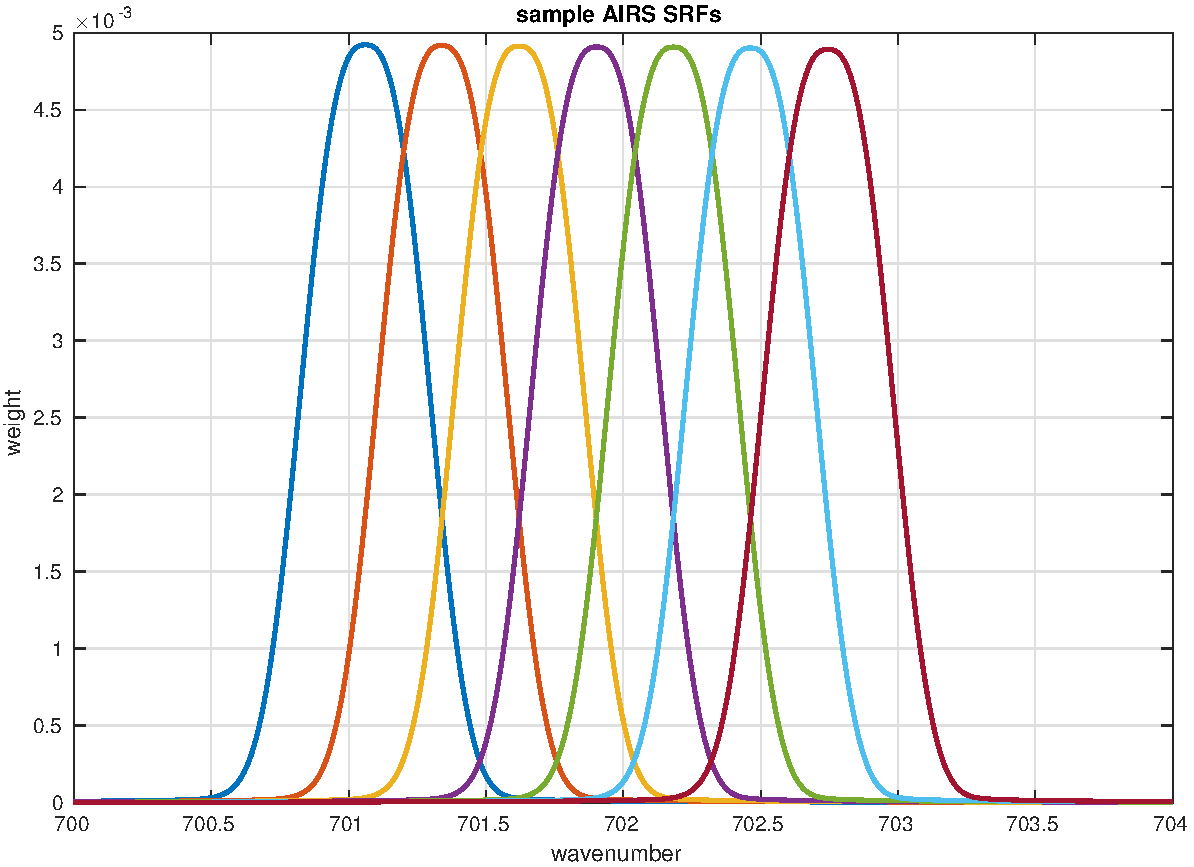
\includegraphics[height=8cm]{figures/airs_sample_SRFs.pdf}
  \caption{sample adjacent {\airs} spectral response functions}
  \label{srfs1}
\end{figure}

\begin{figure} % source plot_SRFs.m
  \centering
  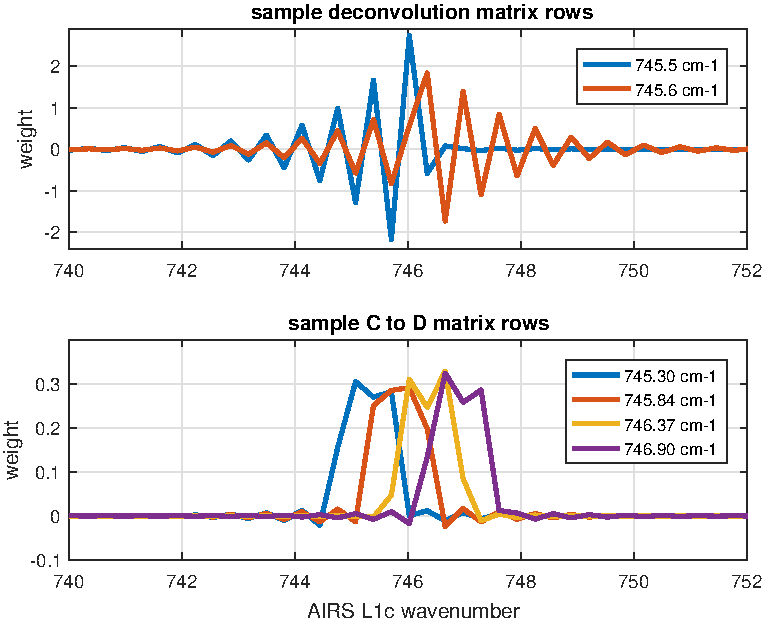
\includegraphics[height=8cm]{figures/airs_decon_basis.pdf}
  \caption{sample basis function for the deconvolved {\airs}
    radiances}
  \label{dbasis}
\end{figure}

\begin{figure} % source cris_test7.m
  \centering
  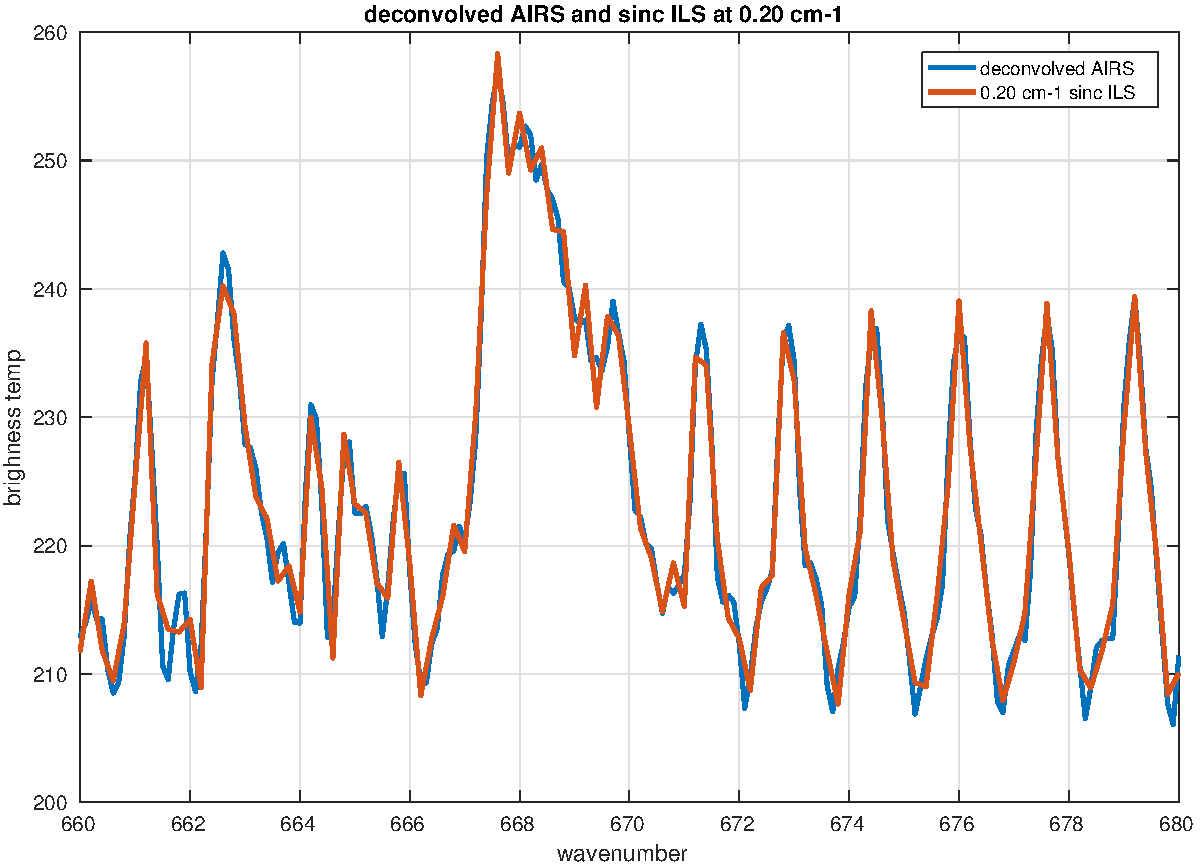
\includegraphics[height=8cm]{figures/airs_decon_res.pdf}
  \caption{detail of deconvolved {\airs} and kcarta 0.0025 {\wn}
    radiances convolved to a sinc ILS at 0.2 {\wn}}
  \label{dsinc}
\end{figure}

Figure \ref{srfs1} shows a typical subset of {\airs} SRFs.  Note the
significant overlap in the wings.  This allows the deconvolution to
recover resolution beyond that of the response functions considered
individually.  The spacing of the AIRS L1b channels is not regular;
there are both gaps and close neighbors, side effects of the focal
plane geometry.  Both the gaps and close neighbors cause problems for
a deconvolution.  The AIRS L1c channel set \cite{airs1c} is a derived
product of the 1b set with filled gaps and relatively regular (though
still frequency dependent) frequency spacing, and we will use the 1c
set here.

Suppose we have $n$ channels and a frequency grid $\vec v$ of $k$
points spanning the domains of the functions $\sigma_i$.  The grid
step size for our applications is often 0.0025 {\wn}, the kcarta
resolution.  Let $S_k$ be an $n\times k$ array such that $s_{i,j} =
\sigma_i(v_j)/w_i$, where $w_i = \sum_j \sigma_i(v_j)$, that is
where row $i$ is $\sigma_i(v)$ tabulated at the grid $\vec v$ and
normalized so the row sum is 1.  If the channel centers are in
increasing order $S_k$ is banded, and if they are not too close the
rows are linearly independent.  $S_k$ is a linear transform whose
domain is radiance at the grid $\vec v$ and whose range is channel
radiances.  If $r$ is radiance at the grid $\vec v$, then $c = S_k r$
gives a good approximation of the channel radiances $c_i = 
\int\sigma_i(v)r(v)\,dv$.

In practice this is how we convolve kcarta or other simulated
radiances to get {\airs} channel radiances.  We construct $S_k$
either explicitly or implicitly from {\airs} {\srf} tabulations.
The matrix $S_k$ in the former case is large but manageable with a
banded or sparse representation.

Suppose we have $S_k$ and channel radiances $c$ and want to 
find $r$, that is, to deconvolve $c$.  Consider the linear system
$S_k x = c$.  Since $n < k$ for the kcarta grid mentioned above this
is underdetermined, with infinitely many solutions.  We could add
constraints, take a pseudo-inverse, consider a new matrix $S_b$ with
columns tabulated at some coarser grid, or some combination of the
above.

For an {\airs} to {\cris} translation we are mainly interested in 
the transform $S_b$ with {\srf}s at an intermediate grid, typically
0.1 {\wn}, the approximate resolution of the {\srf} measurements.
Let $\vec v_b = v_1,v_2,\ldots,v_m$ be a 0.1 {\wn} grid spanning the
domains of the functions $\sigma_i$.  Similar to $S_k$, let $S_b$ be
an $n\times m$ array where row $i$ is $\sigma_i(v)$ tabulated at the
$\vec v_b$ grid, with rows normalized to~1.  If $r$ is radiance at
the $\vec v_b$ grid, then $c = S_b r$ is still a reasonable
approximation of $\int\sigma_i(v)r(v)\,dv$.

Consider the linear system $S_b x = c$, similar to the case 
$S_k x = c$ above, where we are given $S_b$ and channel signals $c$
and want to find radiances $x$.  Since $n < m < k$, as with $S_k$
the system will be underdetermined but more manageable because $m$
is approximately 40 times less than $k$.  We use a Moore-Penrose
pseudoinverse as $S_b^{-1}$.  Then $x = S_b^{-1} c$ gives us
deconvolved radiances at the {\srf} tabulation grid.  Figure
\ref{dbasis} shows a typical basis function for the {\airs}
deconvolution, that is, a column of the pseudo-inverse $S_b^{-1}$.

The {\airs} deconvolution gives a significant resolution enhancement.
Figure \ref{dsinc} shows LW detail of deconvolved {\airs} together
with kcarta radiances convolved directly to a 0.2 {\wn} sinc ILS.
This is not to claim that the deconvolution resolution is 0.2~{\wn}
everywhere, among other things this will depend on the AIRS channel
spacing.  But it is significantly greater than the {\cris} $0.625$
{\wn} LW resolution.  

[ need to look at effective deconvolution resolution for the MW and
  SW bands and to compare this with the $0.625$~{\wn} resolution for
  the {\cris} high resolution mode for those bands ]

\FloatBarrier
\section{AIRS to CrIS translation}
\label{airs2cris}

For the {\cris} standard resolution mode the channel spacing is
$0.625$ {\wn} for the LW, 1.25~{\wn} for the MW, and 2.5~{\wn} for
the SW bands.  The first step in the {\airs} L1c to {\cris}
translation is to deconvolve the {\airs} channel radiances to the
0.1~{\wn} intermediate grid, the nominal {\airs} SRF resolution.
Then for each {\cris} band, we

\begin{itemize}
  \item find the {\airs} and {\cris} band intersection

  \item apply a bandpass filter to the deconvolved {\airs} radiances
    to restrict them to the intersection, with a rolloff outside the
    intersection

  \item reconvolve the filtered spectra to the {\cris} user grid

\end{itemize}

Translations are validated by comparison with calculated reference
truth.  For the results presented in this section we start with 49
fitting profiles spanning a significant range of atmospheric
conditions \cite{sarta1,sarta2}.  Upwelling radiance is calculated
at a 0.0025 {\wn} grid with kcarta \cite{kcarta1} over a band
spanning the {\airs} and {\cris} response functions.  ``True
{\airs}'' is calculated from this by convolving the kcarta radiances
with {\airs} SRFs, and ``true {\cris}'' by convolving kcarta
radiances to the {\cris} instrument specifications.  {\airs} is then
translated to {\cris} to get ``{\airs} {\cris}'', and this is
compared with true {\cris}.  This validation assumes perfect
knowledge of the {\airs} and {\cris} instrument response functions
and so gives only a lower bound on residuals, and on how well the
translations can work in practice.  The better we know the response
functions, the closer real translations can approach these limits.

Figure \ref{specLW} shows true {\cris}, true {\airs}, deconvolved
{\airs}, and {\airs} {\cris}.  In the first subplot we mainly see
the greater fine structure in the deconvolution.  The second subplot
shows details from 660 to 680 {\wn}.  

Figures \ref{diffLW}, \ref{diffMW}, and \ref{diffSW} show the mean
and standard deviation of true {\cris} minus {\airs} {\cris} for the
49 fitting profiles, with and without Hamming apodization, for each
of the {\cris} bands.  Figures \ref{meanAll} and \ref{stdAll}
summarize the mean and standard deviation of the residuals for
Hamming apodized radiances.  The residual has a high frequency
component with a period of 2 channel steps that is significantly
reduced by the apodization.  The constant or DC bias (the mean of
the residuals over frequency) is close to zero for the apodized
residuals: $0.002$~K for the LW, $-0.005$~K for the MW, and
$0.001$~K for the SW.

\begin{figure} % source a2cris_test1
  \centering
  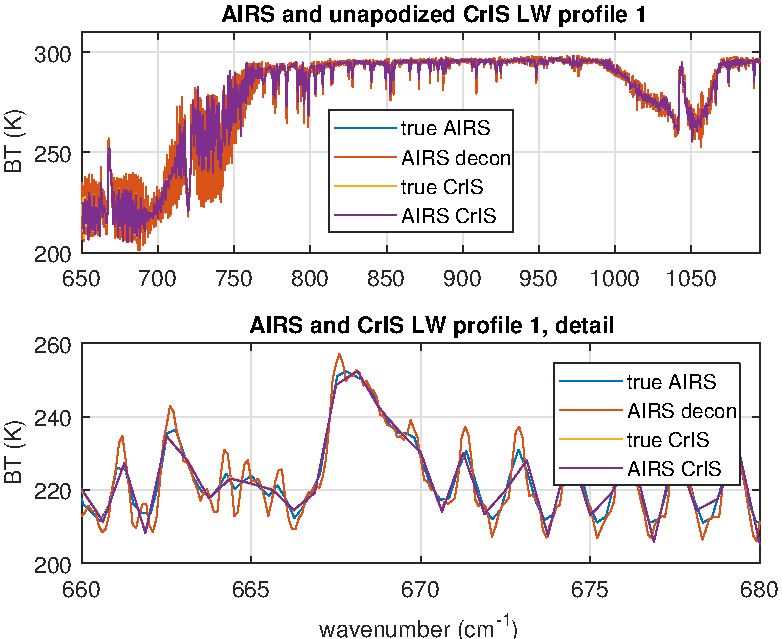
\includegraphics[height=8cm]{figures/a2cris_spec_LW.pdf}
  \caption{true {\cris}, true {\airs}, deconvolved {\airs}, and
    {\airs} {\cris}}
  \label{specLW}
\end{figure}

\begin{figure} % source a2cris_test1
  \centering
  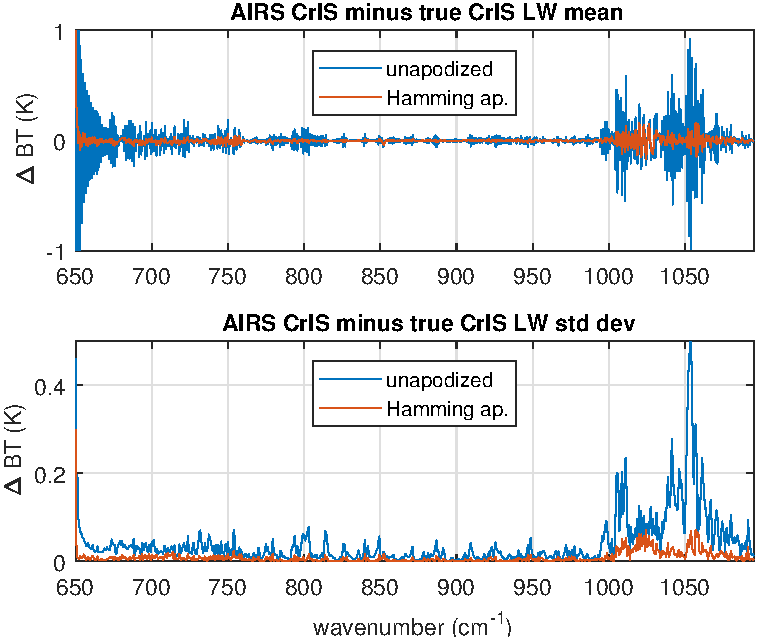
\includegraphics[height=8cm]{figures/a2cris_diff_LW.pdf}
  \caption{Mean and standard deviation of unapodized and Hamming
    apodized {\airs} {\cris} minus true {\cris}, for the {\cris} LW
    band}
  \label{diffLW}
\end{figure}

\begin{figure} % source a2cris_test1
  \centering
  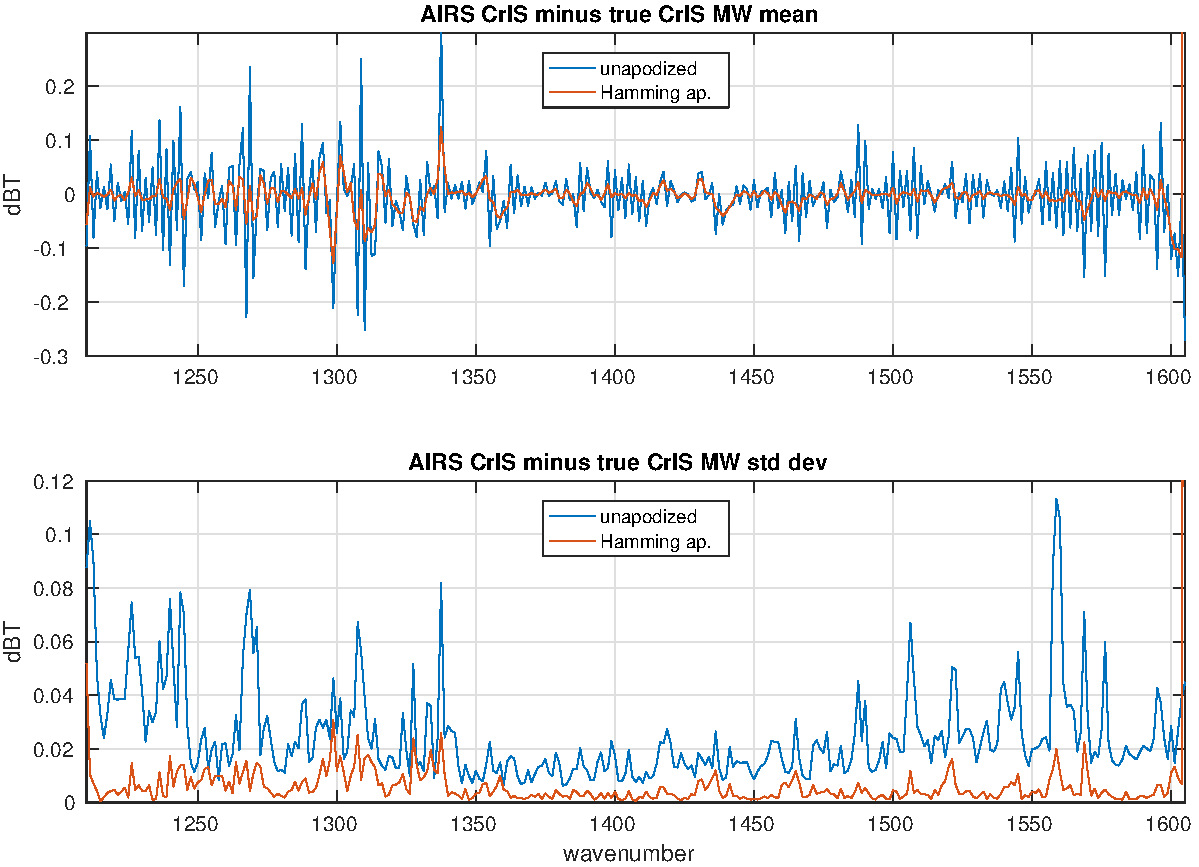
\includegraphics[height=8cm]{figures/a2cris_diff_MW.pdf}
  \caption{Mean and standard deviation of unapodized and Hamming
    apodized {\airs} {\cris} minus true {\cris}, for the {\cris} MW
    band}
  \label{diffMW}
\end{figure}

\begin{figure} % source a2cris_test1
  \centering
  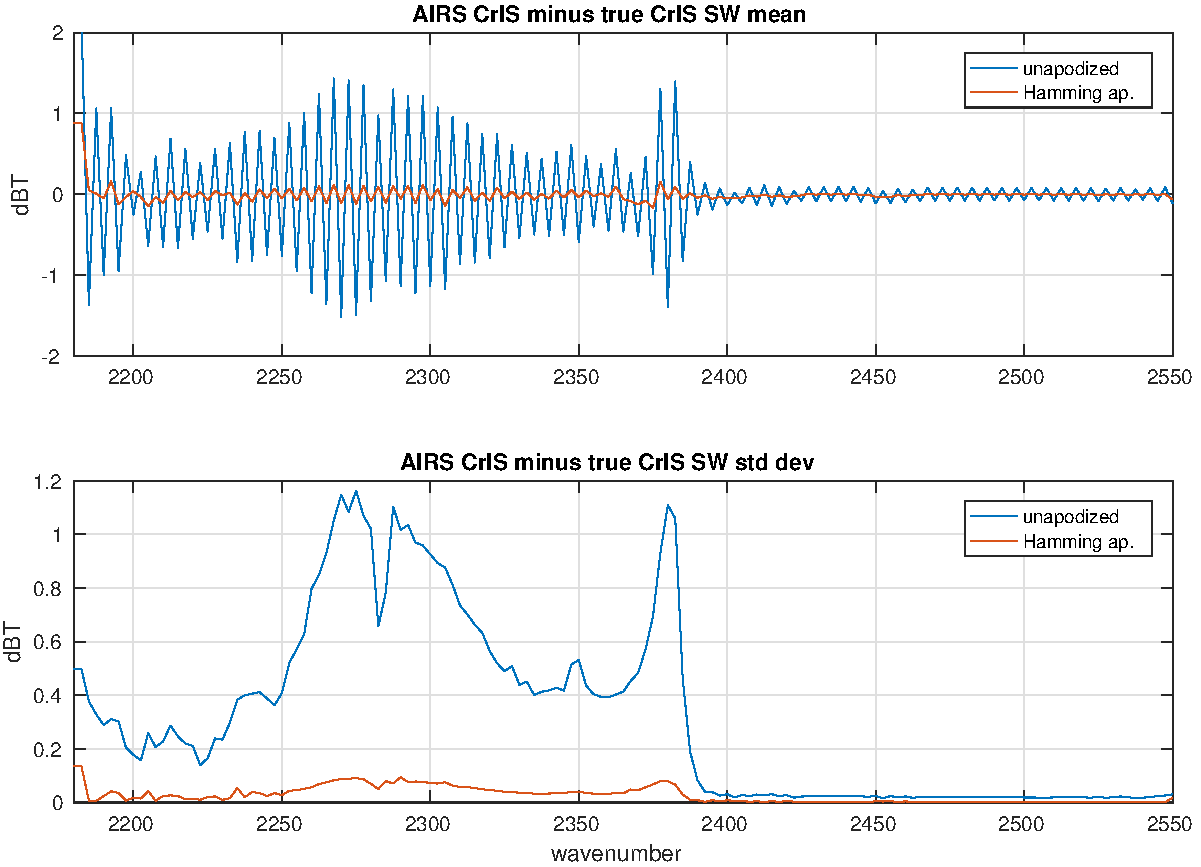
\includegraphics[height=8cm]{figures/a2cris_diff_SW.pdf}
  \caption{Mean and standard deviation of unapodized and Hamming
    apodized {\airs} {\cris} minus true {\cris}, for the {\cris} SW
    band}
  \label{diffSW}
\end{figure}

\begin{figure} % source a2cris_plot2.m
  \centering
  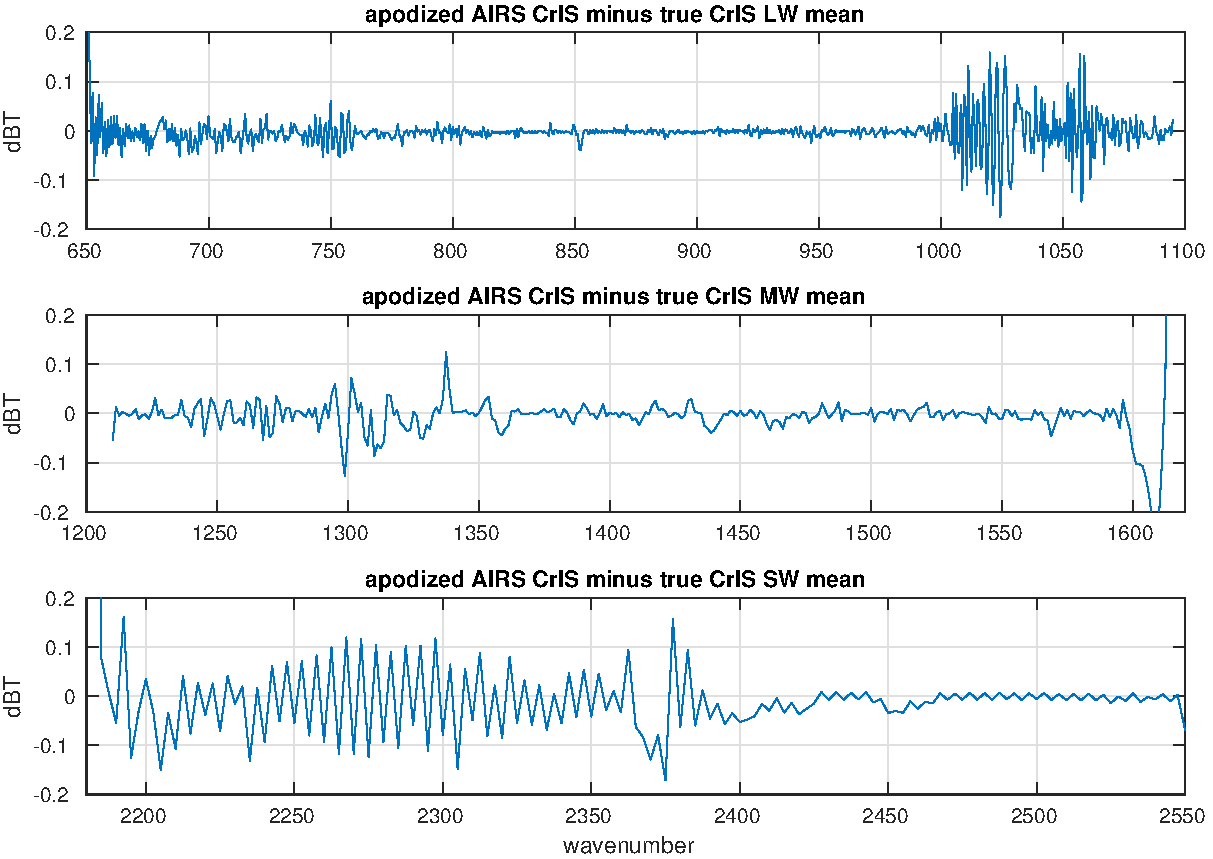
\includegraphics[height=8cm]{figures/combo_ap_dif_mean.pdf}
  \caption{Mean apodized residuals for all three bands}
  \label{meanAll}
\end{figure}

\begin{figure} % source a2cris_plot2.m
  \centering
  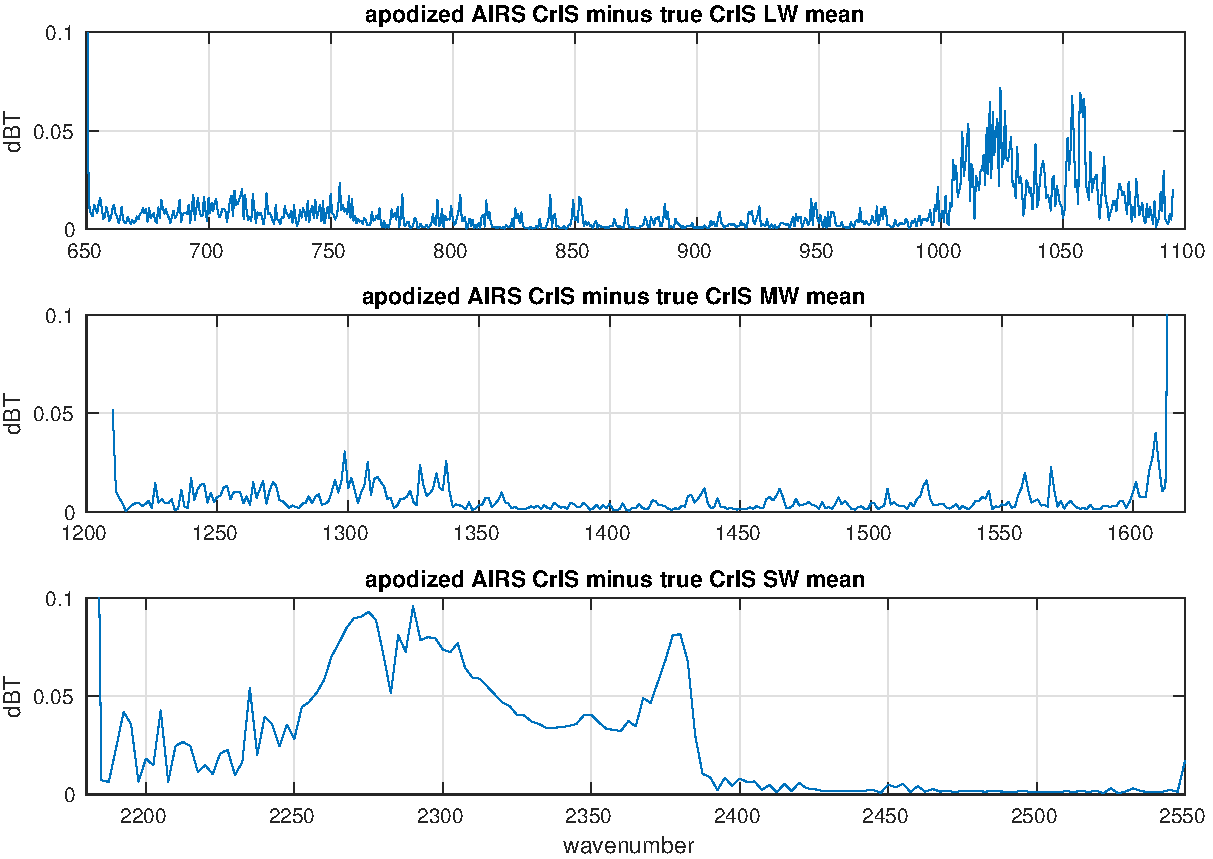
\includegraphics[height=8cm]{figures/combo_ap_dif_std.pdf}
  \caption{Standard deviation apodized residuals for all three bands}
  \label{stdAll}
\end{figure}

\begin{figure} % source a2cris_test1
  \centering
  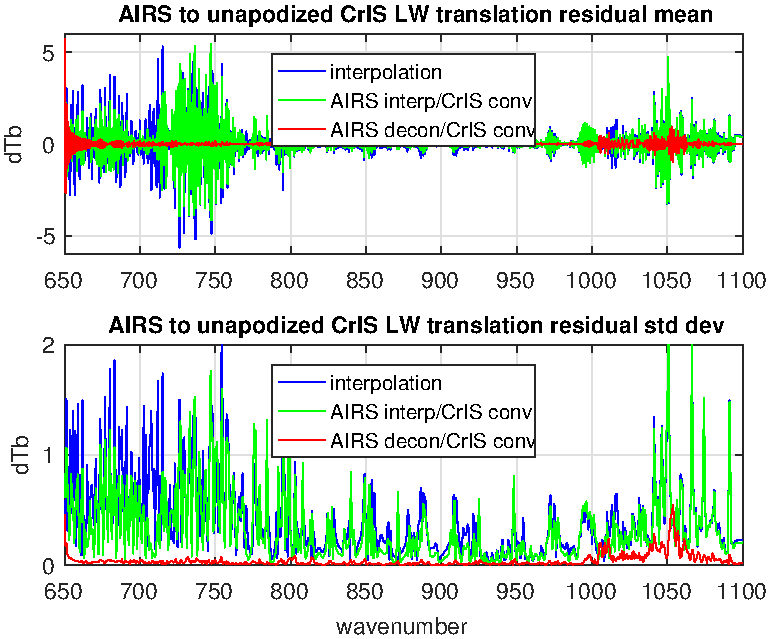
\includegraphics[height=8cm]{figures/a2cris_interp_LW.pdf}
  \caption{spline interpolation, interpolation with convolution, 
    and deconvolution with convolution for the {\cris} LW band}
  \label{intpLW}
\end{figure}

Deconvolution works better than interpolation for the {\airs} to
{\cris} translation.  We consider two cases.  For the first, start
with true {\airs} and interpolate radiances directly to the {\cris}
user grid with a cubic spline.  For the second, interpolate true
{\airs} to the 0.1 {\wn} intermediate grid with a cubic spline and
then convolve this to the use {\cris} user grid.  Figure~\ref{intpLW}
shows interpolated {\cris} minus true {\cris} for the LW band,
without apodization.  The two-step interpolation works a little
better than the simple spline, but both residuals are significantly
larger than for the translation with deconvolution.  Results for the
MW are similar, while the unapodized comparison is less clear for the
SW.  With Hamming apodization, the residuals with deconvolution are
significantly less than interpolation for all three bands.

\FloatBarrier
\section{Statisitcal Refinement}
\label{statfix}

For these tests we start with kcarta radiances calculated from a 
set of 7377 radiances calculated from mostly cloudy AIRS profiles.
These are split randomly into dependent and independent sets.  
Bias or regression coefficients are taken from the dependent set,
and tests are done on the independent set.  As with the 49 profile
set ``true {\airs}'' channel radiances are calculated by convolving
with {\airs} SRFs and ``true {\cris}'' by convolving to the {\cris}
instrument specifications.

Figure \ref{statLW} is a comparison of bias, linear, and quadratic
corrections for a representative dependend/independent partition.
The residuals vary with the partition but the standard deviation is
consistently significantly less for the linear and quadratic cases.
The linear and quadratic corrections are nearly identical, the
quadratic coefficient is very close to zero.  Figure \ref{coefLW}
shows the weights for the linear fits shown above.  The $a$ weight
is very close to 1 and the $b$ weight to earlier bias values.

Figures \ref{statMW} and \ref{statSW} show the linear correction 
is giving a similar significant improvement in the MW standard
deviation in comparison with the LW, and a small improvement in the
SW.  As in the LW the mean residuals vary significantly depending on
the dependent/independent partition, but the standard deviations are
relatively stable.

\begin{figure} % source a2cris_stat4.m
  \centering
  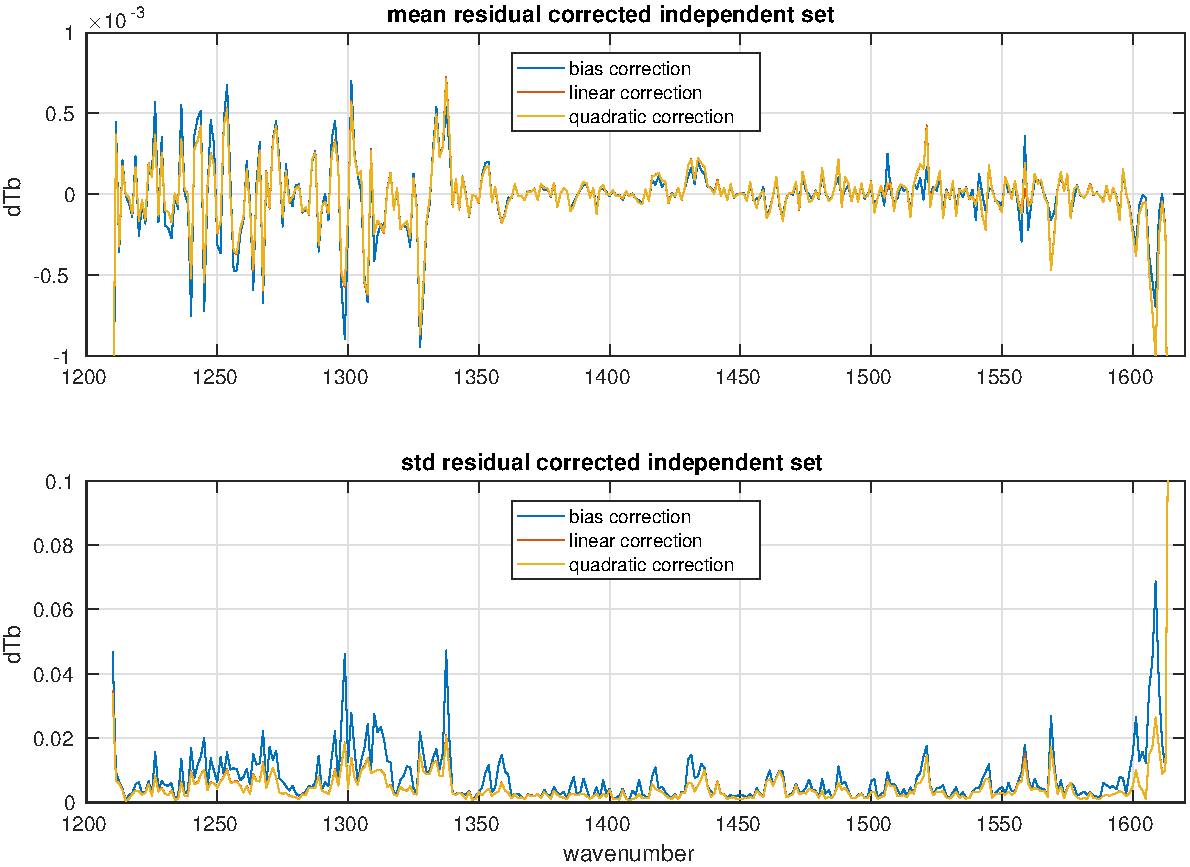
\includegraphics[height=8cm]{figures/a2cris_stat_LW.pdf}
  \caption{Mean and standard deviation of LW corrected apodized
    residuals for the independent subset of the 7377 profile set}
  \label{statLW}
\end{figure}

\begin{figure} % source a2cris_stat4.m
  \centering
  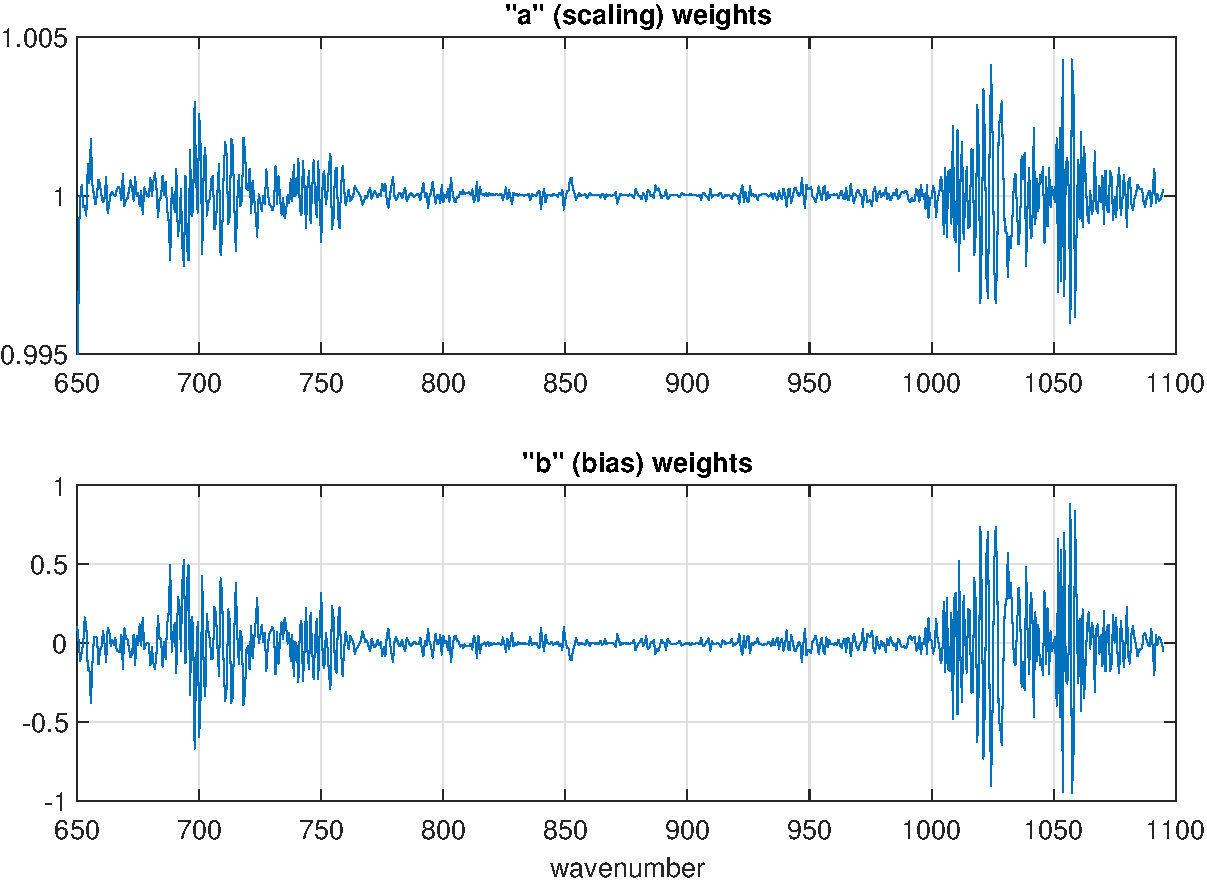
\includegraphics[height=8cm]{figures/a2cris_coef_LW.pdf}
  \caption{LW $a$ and $b$ weights for the linear correction $ax+b$}
  \label{coefLW}
\end{figure}

\begin{figure} % source a2cris_stat4.m
  \centering
  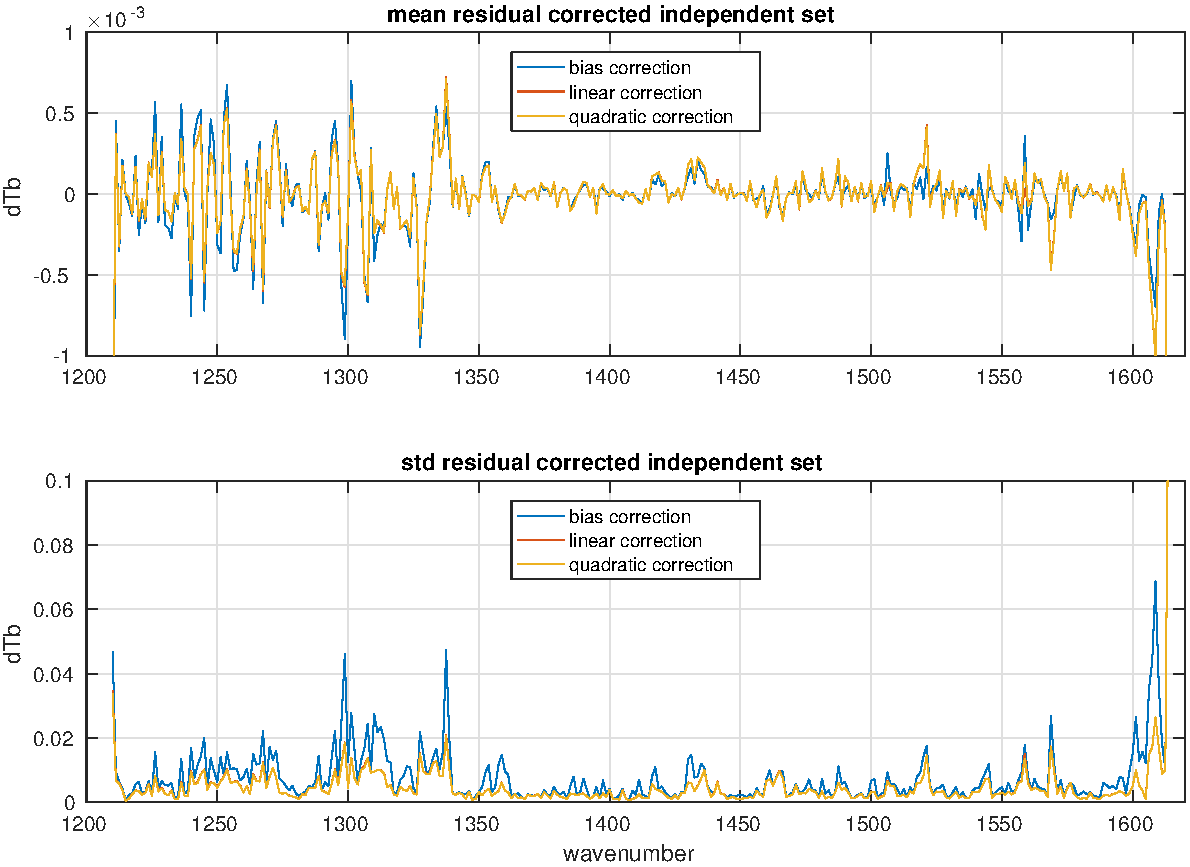
\includegraphics[height=8cm]{figures/a2cris_stat_MW.pdf}
  \caption{Mean and standard deviation of MW corrected apodized
    residuals for the independent subset of the 7377 profile set}
  \label{statMW}
\end{figure}

\begin{figure} % source a2cris_stat4.m
  \centering
  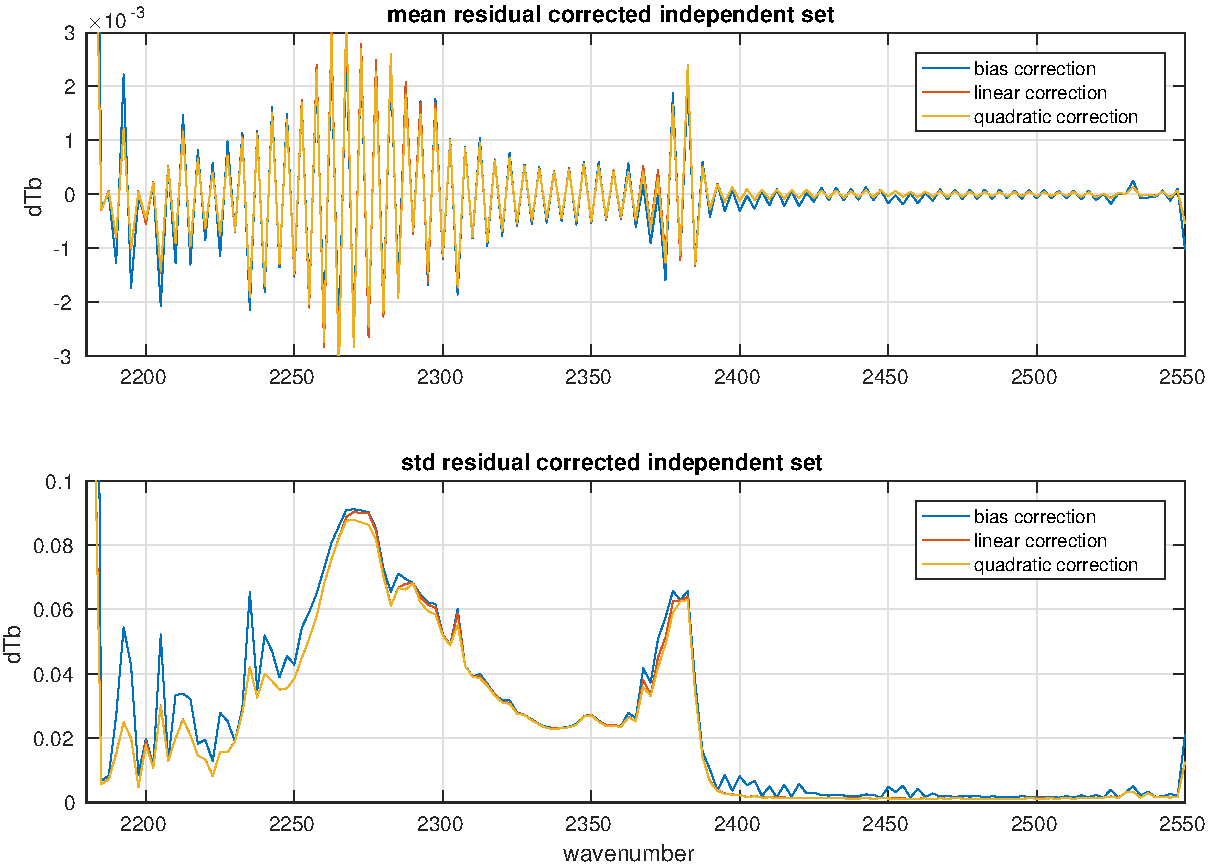
\includegraphics[height=8cm]{figures/a2cris_stat_SW.pdf}
  \caption{Mean and standard deviation of SW corrected apodized
    residuals for the independent subset of the 7377 profile set}
  \label{statSW}
\end{figure}

\FloatBarrier
\bibliographystyle{abbrv}
\bibliography{decon}

\end{document}

